Even with the use of the simulator to get accurate results, it is still necessary to validate the results in real world scenario, for this we need to try and replicate the conditions of that would be found in a space station here on earth. To do this, the Space Cobot robot is fitted with both a gimbal and a base with air bearings, this allows for free rotation in a 3D space, as well as giving the robot the capability of almost frictionless movement in two different axis (XY) when in a special table. The gimbal and air bearing base can be seen in figure \ref{fig:Proposed Approach: Real World: Gimbal and Air bearing base}. With this setup, we can test the robot in a controlled environment, and compare the results againts the expected results from the simulator. Some remarks should be make, with this setup, we can only test the robot in a $R^2 \times \mathbb{SO}(3)$ space, since we cannot move the robot along the Z axis, and the robot is also subject to a pendulum effect whenever the center of mass is not aligned with the gimbal axis. 

\begin{figure}[H]
    \begin{subfigure}{0.5\textwidth}
       \centering
       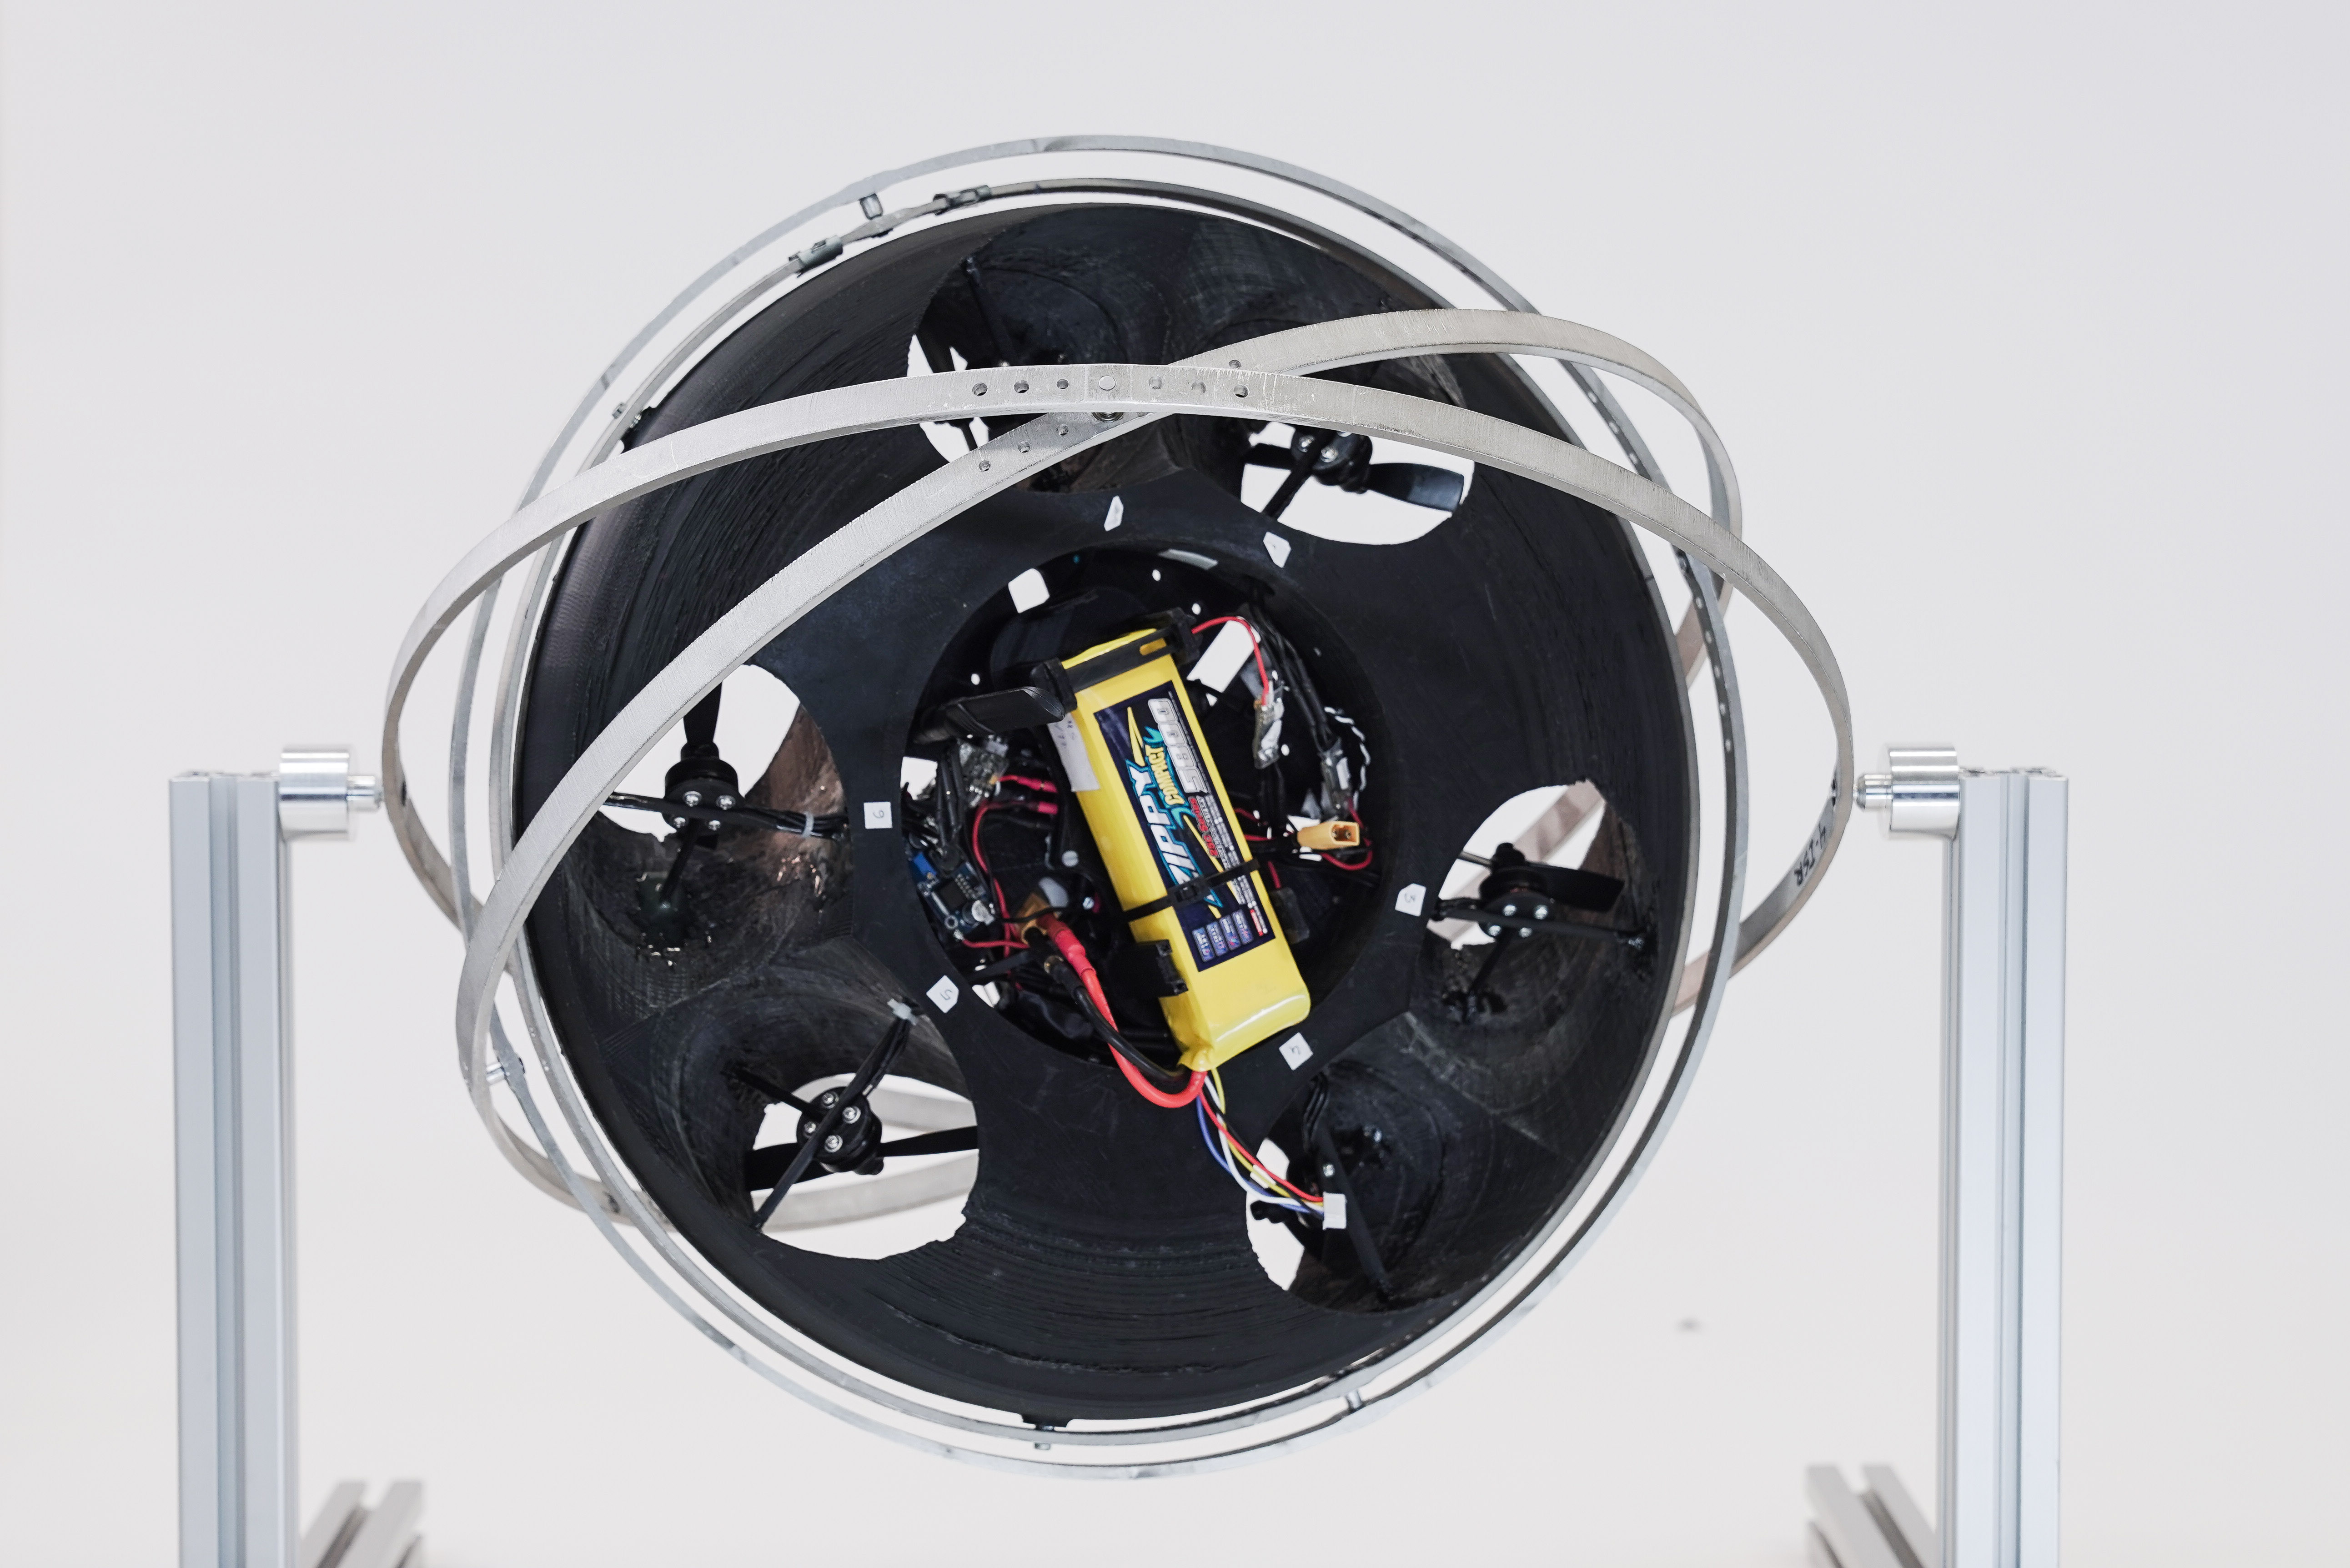
\includegraphics[width=.9\textwidth]{Images/Propposed Aproach/Gimbal.jpg} 
       \caption{Space Cobot Robot assembled inside the gimbal}
       \label{fig: Proposed Approach: Real World: Gimbal}
    \end{subfigure}
    \hfill
    \begin{subfigure}{.5\textwidth}
        \centering
        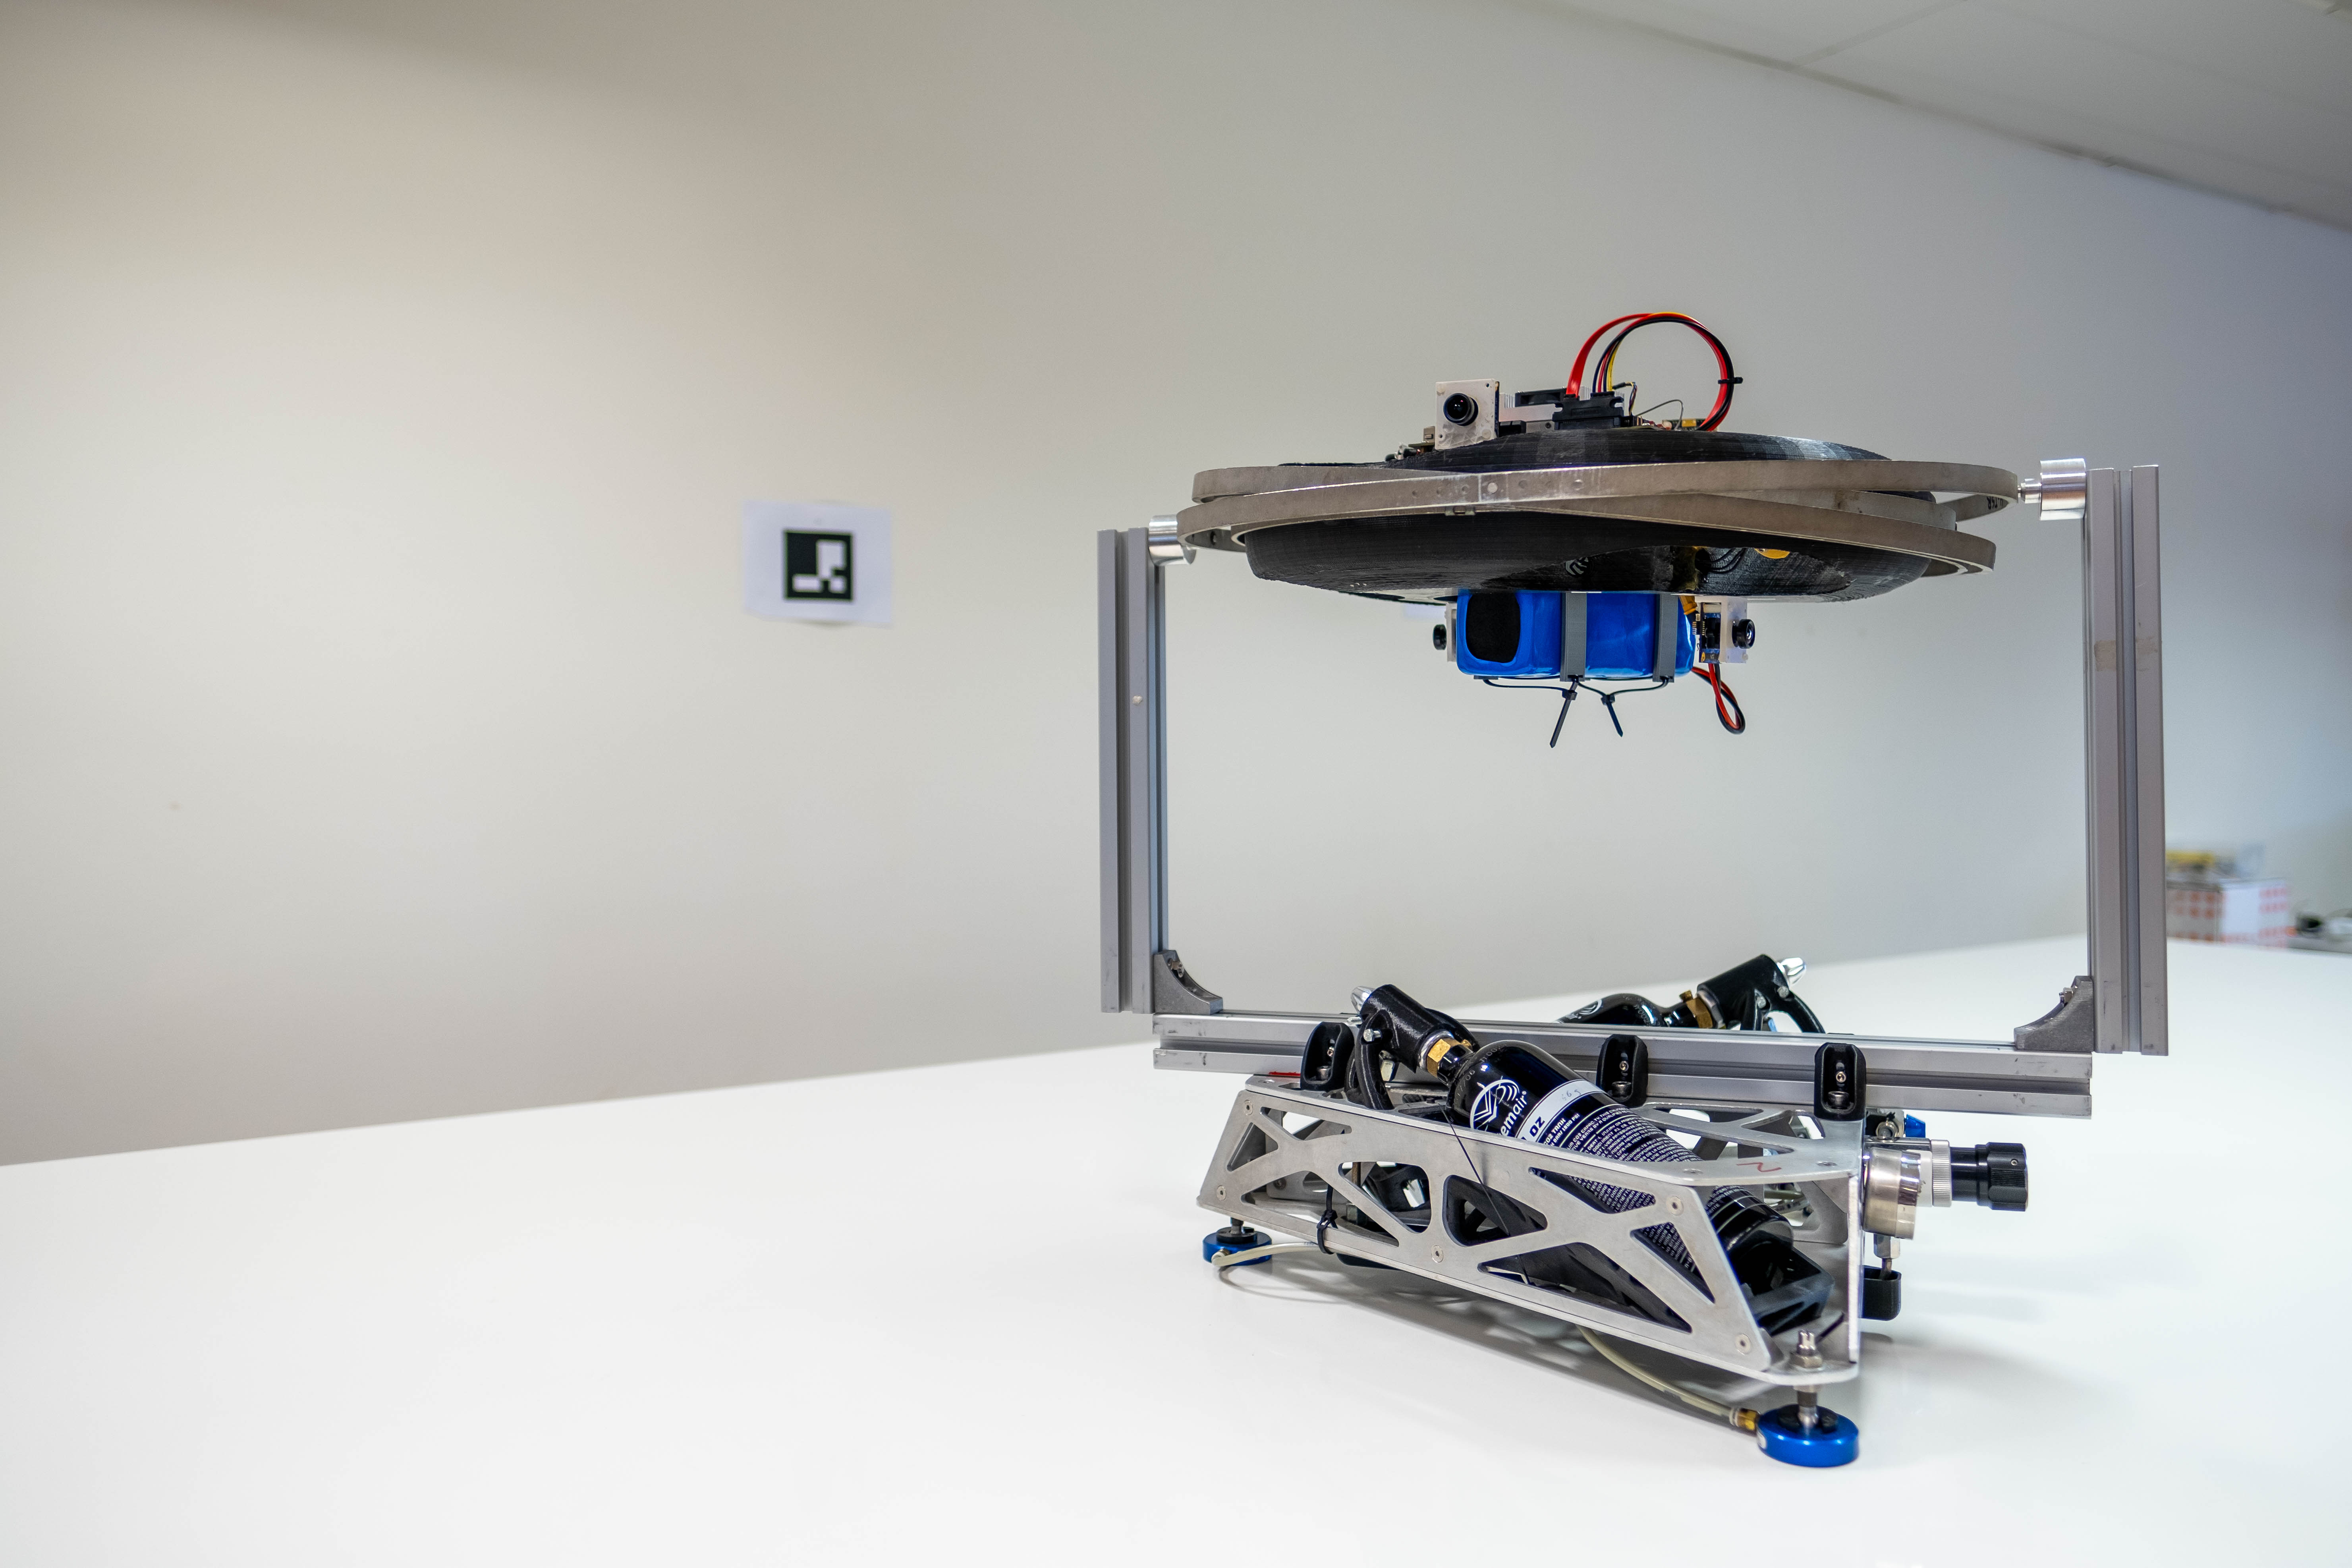
\includegraphics[width=0.9\textwidth]{Images/Propposed Aproach/Air Bearing .JPG}
        \caption{Space Cobot Robot assembled on the air bearing base}
        \label{fig: Proposed Approach: Real Word: Air Bearings}
    \end{subfigure}
    \caption{Space Cobot Robot assembled on the gimbal and air bearing base}
    \label{fig:Proposed Approach: Real World: Gimbal and Air bearing base}
\end{figure}